
\section{Premessa}
\label{sec:premessa}
Prima di proseguire con la lettura del documento è bene puntualizzare alcune cose.
Innanzitutto va ricordato che il nostro prodotto consta di due plugin \emph{distinti} che svolgono funzioni diverse, ma che comunque interagiscono con i dati presenti sul server ElasticSearch in modo simile. Per semplificare la rappresentazione grafica e per evitare ripetizioni essi sono stati, in questa fase di progettazione, considerati come facenti parte dello stesso sistema. Questo è reso possibile dall'alta sovrapposizione di componenti necessari al loro funzionamento. Tuttavia, nella fase di produzione, essi verranno completamente disaccoppiati e saranno presentati come due plugin distinti che avranno delle parti in comune, che per come è progettato Kibana, dovranno essere per necessariamente ripetute. Va segnalato che il linguaggio di programmazione da noi usato, Javascript, è \emph{weakly typed}. Questo comporta. ad esempio, poca precisione per quanto riguarda il tipaggio dei parametri passati ai metodi. Per questo, soprattutto nella fase di rappresentazione grafica delle classi del sistema, ci terremmo talvolta vaghi sul tipo dei parametri passati e ritornati da metodi. Tali imprecisioni verranno tuttavia chiarite nella parte di testo che riguarda ogni specifico componente. Inoltre, esserendo ElasticSearch un database non relazionale i dati da esso ritornati non hanno una struttura fissa, dunque molte volte verranno descritti semplicemente come \texttt{Array} o \texttt{Object}, chiarendo nella descrizione testuale di che tipo di aray o oggetto si tratta.

\section{Componenti}

Ogni plugin per Kibana è articolato in due sezioni principali: lato client e lato server. Si presenta di seguito il dettaglio di ciasuna sezione.

\subsection{Lato Server}
Il lato server si deve occupare di interrogare il database Elasticsearch ed esporre i risultati delle query tramite API REST al lato client.

\subsubsection{Design lato server}
Le funzioni che il lato server può compiere sono \emph{volutamente}  poche e basilari. La scelta progettuale di spostare sul lato client tutta la parte di elaborazione del dato è stata dettata da necessità tecniche: i plugin di Kibana vengono eseguiti all'interno di un'istanza del server Kibana. Spesso essi sono installati su server AWS con una limitata capacità di calcolo, molte volte 2GB di memoria RAM. Per questo motivo se avessimo eseguito elaborazioni complicate e impegnative su tali macchine ci sarebbe stato il rischio che con l'aumentare dell'utenza il servizio sarebbe potuto essere lento. Spostando lato client tali elaborazioni il servizio offerto diventa scalabile.

\subsubsection{Rappresentazione}
Nel seguente diagramma delle classi, figura \ref{img:diagrammaClassiServer}, ciascuna API viene rappresentata tramite una classe composta da un singolo metodo. Tale metodo intende rappresentare il funzionamento della API. Ciascuna di esse è interrogabile dal lato client tramite una richiesta GET.


\begin{figure}[H]
	\centering
	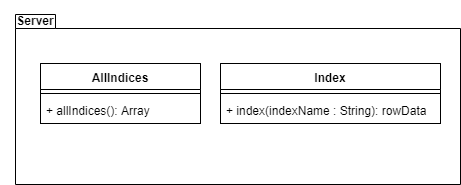
\includegraphics[width=1\textwidth]{Images/DiagrammaClassiServer.png}
	\caption{Diagramma UML delle classi riguardanti il lato server}
	\label{img:diagrammaClassiServer}
\end{figure}

\subsubsection{AllIndices}
AllIndices è la API che si occupa di restituire al chiamante la lista di \emph{tutti} gli indici presenti all'interno della istanza di Elasticsearch collegata. La lista degli indici è un array di stringhe contenente per ogni indice il proprio nome.

\subsubsection{Index}
Index è la API che espone l'interfaccia per poter leggere i dati contenuti all'interno di un indice. Nella richiesta GET deve essere specificato un parametro chiamato index, il cui valore rappresenta l'indice del quale si vogliono ottenere i dati. Ciò che viene ritornato al richiedente è un oggetto \emph{grezzo}, ovvero la risposta dell'istanza Elasticsearch, con tutti i dati amministrativi che Elasticsearch utilizza annessi (e.g. campi preceduti da underscore, \texttt{"\_id"}). Sarà compito del client reperire le informazioni a lui utili

\subsection{Lato Client}
Il lato client si occupa di interrogare il lato server per ottenere informazioni grezze, elaborarle per renderle utili ed infine presentarle all'utente.

\label{sec:Componenti}
\subsubsection{Rappresentazione}
Il codice prodotto è stato scritto in Javascript ES6, quindi molti concetti quali classi ed interfacce non sono presenti all'interno del linguaggio. Per produrre un diagramma delle classi dunque sono state considerate \emph{ classi } sia oggetti Javascript, sia funzioni e talvolta costrutti più complessi. Tali stratagemmi verranno comunque chiariti nella descrizione testuale di ciascun componente. Per quanto riguarda le interfacce che sono presenti nel diagramma delle classi, figura \ref{img:diagrammaClassiClient}, nel codice non sono effettivamente presenti tali interfacce, ma tutte le classi che implementano tale interfaccia \emph{devono} possedere i metodi esposti da tale interfaccia. Questo stratagemma è stato particolarmente utile nell'implementazione del componente \texttt{DataCleaner}, come descritto in \ref{sec:DataCleaner}.

\begin{figure}[H]
    \centering
    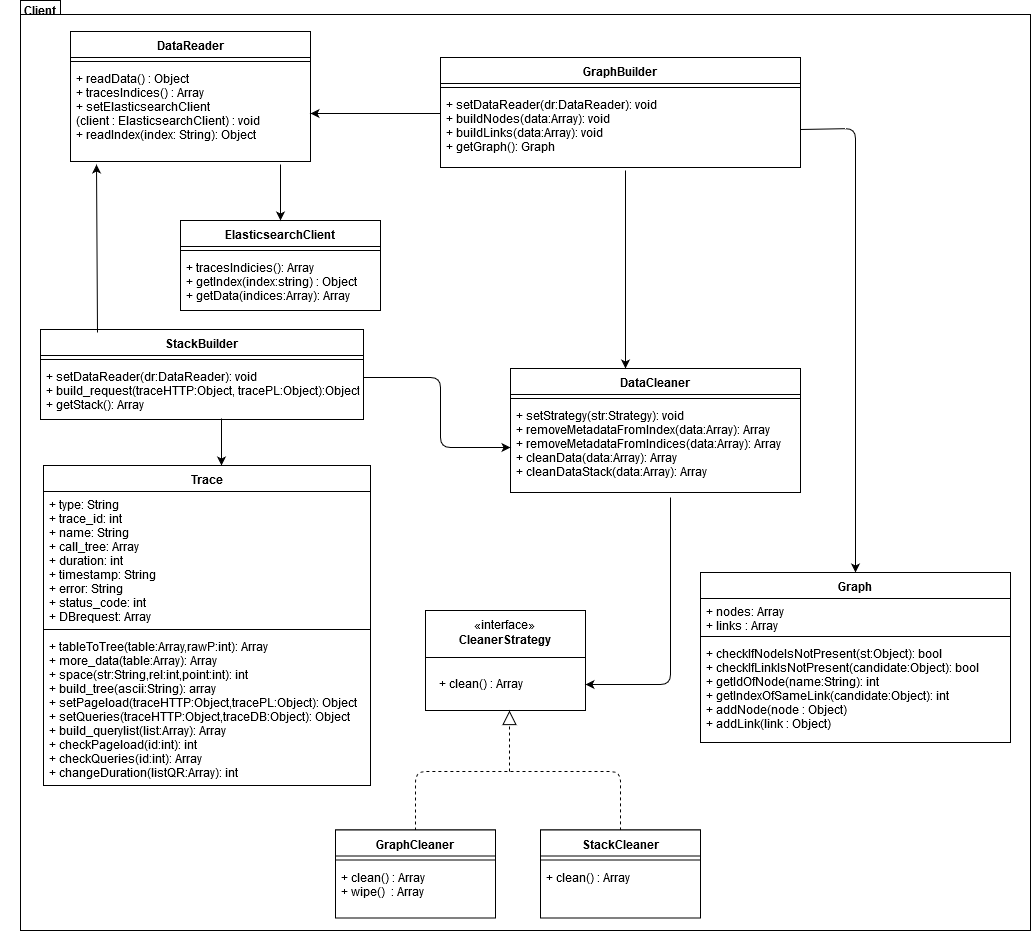
\includegraphics[width=1\textwidth]{Images/classi.png}
    \caption{Diagramma delle classi dell'applicazione}
    \label{img:diagrammaClassiClient}
\end{figure}

\subsubsection{ElasticsearchClient} 
\texttt{ElasticsearchClient} è il componente che si occupa di fare le chiamate API al lato server. Non è una classe vera e propria all'interno del codice, ma un \emph{Service}. 
I Service sono funzioni, od oggetti, che possono essere passati a tutte le altri componenti di angularJs attraverso Dependency Injection, permettono di condividere codice e funzionalitá facilmente. Essi sono \emph{lazily instantiated}, cioé generati solo quando un componente esprime una dipendenza verso un determinato service e realizzano il design pattern "singleton". Permettono la realizzazione di servizi come i client API, dove avere piú istanze dello stesso client non sarebbe ragionevole. 
Utilizzare un service è l'unico modo per poter eseguire chiamate REST parametrizzate al lato server. Ciascun metodo qui presentato nasconde in realtà una chiamata GET all'opportuno componente lato server. I metodi da esso esposti sono: 
\begin{itemize} 
  \item \texttt{tracesIndices()} ritorna un array di stringhe che rappresenta gli indici contenuti nell'istanza di ElasticSearch che hanno all'interno delle traces; 
  \item \texttt{getIndex(index)} ritorna al chiamante i dati grezzi che vengono restituiti da Elasticsearch eseguendo una ricerca priva di parametri sull'indice passato come parametro, ovvero \texttt{index}. Essi comprendono, oltre tutti i documenti dell'indice, anche i metadati di Elasticsearch; 
  \item \texttt{readData()}: ritorna al chiamante un array di dati grezzi, ognuno dei quali rappresenta il risultato di una ricerca priva di parametri su un indice. Gli indici letti sono quelli ritornati da \texttt{tracesIndices()}, ovvero tutti e soli quelli che contengono traces. 
\end{itemize} 
Osserviamo che anche se in questa rappresentazione questi metodi sono all'interno di un oggetto, non avendo i diagrammi delle classi UML un costrutto per rappresentare precisamente un \emph{service}, essi non hanno una struttura ben definita e oggetti di tipo \texttt{ElasticsearchClient} chiaramente non sono istanziabili. Dunque, per interfacciarsi ad Elasticsearch si è deciso di racchiudere tutte queste funzionalità in un oggetto vero e proprio, \texttt{DataReader} (descritto nella sezione \ref{sec:DataReader}), per poter avere una più agevole interazione con i dati. 
 

\subsubsection{DataReader}
\label{sec:DataReader}
\texttt{DataReader} è il componente del sistema che si occupa di reperire i dati da Elasticsearch, ciò viene fatto utilizzando il \emph{service} \texttt{ElasticsearchClient}. Sarebbe effettivamente possibile utilizzare le chiamate al \emph{service} ogni qualvolta fossero necessari dei dati, tuttavia ricordiamo che tali chiamate non vengono racchiuse all'interno di un oggetto ben strutturato, ma sono un \emph{service}. Restituirà ai richiedenti le informazioni grezze, esattamente come vengono restituite da Elasticsearch. I metodi sono: 
 

\begin{itemize}
	\item \texttt{setElasticsearchClient(client)}: permette di impostare una sorgente dei dati;
	\item \texttt{tracesIndices()}: ritorna un array di stringhe, i quali elementi sono tutti e soli gli indici all'interno dell'istanza di Elasticsearch che hanno al loro interno delle traces. Ciò viene realizzato tramite una chiamata al lato server all'API \texttt{AllIndices} e dunque vengono tenuti solo indici che contengono nel nome la sottostringa \emph{spans};
	\item \texttt{readIndex(index)}: ritorna al chiamante i dati grezzi che vengono restituiti da Elasticsearch eseguendo una ricerca priva di parametri sull'indice passato come parametro, ovvero \texttt{index}. Essi comprendono oltre tutti i documenti dell'indice anche i dati amministrativi di Elasticsearch;
	\item \texttt{readData(indices)}: ritorna al chiamante un array di dati grezzi, ognuno dei quali rappresenta il risultato di una ricerca priva di parametri su un indice. Gli indici letti sono quelli passati tramite parametro.


\end{itemize}



\subsubsection{DataCleaner}

\label{sec:DataCleaner}
\texttt{DataCleaner} è il componente del sistema che si occupa di pulire i dati grezzi che sono stati reperiti da ElasticSearch. Esso compie questo lavoro in due tempi: prima estraendo i dati "utili" da Elasticsearch e poi pulendoli attraverso una \emph{strategy}, descritta in \ref{sec:CleanerStrategy}.\\
I suoi metodi sono:
\begin{itemize}
	\item \texttt{removeMetaDataFromIndex(Array)} il quale si occupa di rimuovere i metadati di Elasticsearch che sono presenti in un singolo indice che gli è passato come input sotto forma di Array. Questo metodo ritorna un array contenente i documenti JSON così come essi sono stati inseriti dall'applicazioni di monitoring negli indici di ElasticSearch. ElasticSearch, infatti, immagazzina i documenti JSON nel campo \texttt{\_source} il quale è inserito in oggetti che contengono altri dati ed informazioni "di servizio". Il metodo si occupa di rimuovere questi dati e costruisce un array contenente il solo contenuto dei campi \texttt{\_source}.
	\item \texttt{removeMetaDataFromIndices(Array)} il quale si occupa di rimuovere i metadati di ElasticSearch da un Array di indici invocando il metodo \texttt{removeMetaDataFromIndex(Array)} su ognuno dei singoli indici.
	\item \texttt{cleanData(Array)} il quale chiama l'implementazione di clean della strategia che possiede sull'array di dati che è stato ritornato dal metodo \texttt{removeMetaDataFromIndeces(Array)}  Tale strategia è incaricata di raffinare ulteriormente i dati per la costruzione della Mappa Topologica oppure per la costruzione dello Stack Trace tramite il metodo \texttt{clean(data)}.
	\item \texttt{cleanDataStack(Array)} il quale chiama l'implementazione di clean della strategia che possiede sull'array di dati che è stato ritornato dal metodo \texttt{removeMetaDataFromIndex(Array)}.
	\item \texttt{setStrategy(Object)} il quale riceve in input un oggetto che implementa l'interfaccia \texttt{CleanerStrategy} e lo assegna al riferimento proprio dell'oggetto.
	
\end{itemize}
Risulta chiaro che esiste dunque una dipendenza fra la struttura dei dati che vengono restituiti da ElasticSearch, la classe \texttt{DataCleaner} e le classi che implementano \texttt{CleanerStrategy}. Tuttavia, i client di \texttt{DataCleaner} potranno avere accesso diretto ai dati di ElasticSearch, privi di dati amministrativi.

	
\subsubsection{CleanerStrategy}
\label{sec:CleanerStrategy}
\texttt{CleanerStrategy} è l'interfaccia che verrà implementata per realizzare una pulizia più raffinata dei dati di un \texttt{DataCleaner}. Espone il metodo \texttt{clean(data)}, che avrà comportamenti diversi a seconda della strategia che si desidera applicare. Dato che il prodotto è implementato in Javascript il costrutto interfaccia non è presente nel linguaggio. Per ovviare a questa mancanza tutte le classi che dovrebbero implementare questa interfaccia \emph{devono} possedere un metodo \texttt{clean(data)} che funzioni come ci si aspetti. 

	
	
\subsubsection{GraphCleaner}
\label{sec:GraphCleaner}

\texttt{GraphCleaner} è l'implementazione di \texttt{CleanerStrategy} utilizzata da \texttt{DataCleaner} per pulire i dati che dovranno essere utilizzati per la costruzione del grafo rappresentante la mappa topologica. Esso dispone dei seguenti metodi:
\begin{itemize}
	\item \texttt{wipe(Array)} che riceve come input un Array che contiene i documenti JSON di un indice. Esso scorre tale Array e ritorna un Array contenente l'insieme di documenti all'interno dell'indice che rappresentano richieste di dati ai database dell'applicazione oppure ai server, ovvero il sottoinsieme di documenti che serviranno effettivamente per la costruzione del grafo;
	\item \texttt{clean(Array)} che riceve come imput un Array di indici che contengono al loro interno i documenti JSON sottoforma di Array. Tale metodo agisce scorrendo l'array che riceve invocando il metodo \texttt{wipe(Array)} su ogni sottoarray.
\end{itemize}

\subsubsection{StackCleaner}
\label{sec:StackCleaner}

\texttt{StackCleaner} è l'implementazione di \texttt{CleanerStrategy} utilizzata da \texttt{DataCleaner} per pulire i dati che dovranno essere utilizzati durante la costruzione della stack trace. Essa dispone del metodo
\begin{itemize}
	\item \texttt{clean(data)} il quale scorre tutti i documenti JSON disponibili ed ha come output l'insieme di documenti che rappresentano chiamate HTTP, JDBC oppure Pageload, ovvero tutte e sole quelle necessarie per la costruzione dei dati strutturati della stack trace.
\end{itemize}

\subsubsection{Trace}
\label{sec:Trace}
\texttt{Trace} rappresenta una richiesta che viene fatta al sistema contenente solo i dati veramente utili alla successiva costruzione della Stack Trace. Questi sono:
\begin{itemize}
	\item \texttt{type}: che riconduce ad una delle tipologie di trace;
	\item \texttt{trace\_id}: numero univoco che permette l'associazione tra trace HTTP, JDBC e Pageload;
	\item \texttt{name}: identificazione generale della richiesta;
	\item \texttt{call\_tree}: array contenente gerarchicamente la lista dei metodi invocati dall'applicazione per compiere la richiesta;
	\item \texttt{duration}: tempo impiegato dal sistema per lo svolgimento della richiesta, compreso il tempo dei metodi, delle query e del caricamento della pagina;
	\item \texttt{timestamp}: data e ora dello svolgimento della richiesta;
	\item \texttt{error}: presenza o meno di errori;
	\item \texttt{status\_code}: tipologia di errore;
	\item \texttt{DBrequest}: (opzionale) array contenente le query con cui è stato interrogato il database.
\end{itemize}
 La tipologia delle trace viene identificata tramite i metodi \texttt{checkPageload()} e \texttt{checkQueries()} e queste possono essere:
	\begin{itemize}
	\item HTTP: insieme di metodi scatenati da un evento generico;
	\item HTTP + Pageload: insieme di metodi scatenati dal caricamento di una pagina web;
	\item HTTP + JDBC + Pageload: insieme di eventi che portano all'interrogazione di un database e che provocano un successivo caricamento di una pagina.
	\end{itemize}
Inoltre i dati vengono calcolati in base alla tipologia della trace tramite  \texttt{setPageload()} e  \texttt{setQueries()} che utilizzano determinate funzioni per la manipolazione dei dati:
\begin{itemize}
	\item Per il campo \texttt{call\_tree} avviene un'accurata manipolazione attraverso il metodo \texttt{build\_tree()} per passare da un tipo stringa ad una gerarchia di oggetti.
	Al metodo \texttt{build\_tree()} viene passato il dato sotto forma di stringa in cui, attraverso l'ASCII art, viene rappresentato un albero dei metodi che vengono invocati con delle informazioni particolari per ognuno di essi. Questo utilizza a sua volta il metodo \texttt{more\_data()} per costruire un array bidimensionale che elenca tutti i metodi e per ognuno ne specifica i dati aggiuntivi rappresentati dall'ASCII art (come total time e self time), il grado di indentazione nell'albero, il numero di metodi figli e il numero di metodi discendenti da esso. \\ Da questa struttura il metodo \texttt{tableToTree()} ricava un oggetto con innestati altri oggetti rappresentanti i metodi e i propri dati strutturati in maniera da rispecchiare i legami di parentela dell'ASCII art.
	\item 	Il metodo \texttt{change\_duration} permette di far variare il tempo di esecuzione delle richieste in base alla tipologia in quanto per ognuna bisognerà considerare più parametri per calcolare i millisecondi impiegati.
\end{itemize}

\subsubsection{StackBuilder}
\label{sec:StackBuilder}

\texttt{StackBuilder} si occupa della creazione della struttura della stack trace per la sua successiva visualizzazione.
Esso viene istanziato con un oggetto \texttt{DataReader} per poter ottenere i dati.
Il metodo principale è \texttt{getStack()} che controlla tutte le chiamate HTTP ricevute dal \texttt{DataReader} e pulite dal \texttt{DataCleaner}, creato e istanziato con strategia \texttt{StackCleaner}, creando delle \texttt{Trace} da ogni richiesta con dati grezzi.

\subsubsection{Graph}
\label{sec:Graph}
	\texttt{Graph} è il tipo di dato che rappresenta il grafo della mappa topologica dell'applicazione. Esso contiene due Array, uno chiamato \texttt{Nodes} e uno chiamato \texttt{Links}.
	\label{sec:Nodes}
	L'Array di \texttt{Nodes} contiene degli oggetti, detti \texttt{Node} rappresentanti i nodi della mappa che contengono i seguenti campi:
	\begin{itemize}
		\item \texttt{id}, contiene un id numerico intero univoco che individua un nodo;
		\item \texttt{name}, contiene il nome del nodo che verrà visualizzato nella mappa. Anche esso è univoco;
		\item \texttt{type}, contiene la tipologia del nodo, che potrà essere ad esempio Server oppure Database.
	\end{itemize}
	\label{sec:Links}
	L'Array di \texttt{Links} contiene oggetti che rappresentano la di comunicazione tra due \texttt{Node} e contengono i seguenti campi:
	\begin{itemize}
		\item{\texttt{source}, che rappresenta il nodo che ha effettuato la chiamata sotto forma di id numerico intero;}
		\item{\texttt{target}, che rappresenta il nodo che ha ricevuto la chiamata sotto forma di id numerico intero;}
		\item{\texttt{type}, che può essere "Database" o "HTTP", per rappresentare i diversi tipi di comunicazione;}
		\item{\texttt{average\_response\_time}, che contiene il tempo medio di risposta di tutte le trace tra source e target;}
		\item{\texttt{number\_of\_requests}, che serve per mantenere consistente il campo \texttt{average\_response\_time}.}
	\end{itemize}
	Esso è individuato univocamente dalla coppia di campi \texttt{source} e \texttt{target}.
	Il tipo di dato \texttt{Graph} contiene i seguenti metodi:
	\begin{itemize}
		\item{\texttt{checkIfNodeIsNotPresent(Object)} controlla se l'oggetto che gli viene passato, che è assunto essere un \texttt{Node} risulta già essere presente nell'Array \texttt{Nodes} attraverso un controllo sul campo \texttt{name}; }
		\item{\texttt{checkIfLinkIsNotPresent(Object)} controlla se l'oggetto che gli viene passato, che è assunto essere un \texttt{Link} risulta già essere presente nell'Array \texttt{Links} attraverso un controllo sulla coppia di campi \texttt{source} e \texttt{target}; }
		\item{\texttt{getIdOfNode(String)} scorre l'Array \texttt{Nodes} finchè non trova un \texttt{Node} con campo \texttt{name} uguale a quello passatogli come parametro; }
		\item{\texttt{getIndexOfSameLink(Object)} scorre l'Array \texttt{Links} finchè non trova un \texttt{Link} con campi \texttt{source} e \texttt{target} uguali a a quelli dell'oggeto che gli è passato, che è assunto essere un \texttt{Link};}
		\item{\texttt{addNode(Object)} aggiunge l'oggetto passatogli, che è assunto essere un \texttt{Node} all'Array \texttt{Nodes}, se esso non è già presente;}
		\item{\texttt{addLink(Object)} aggiunge l'oggetto passatogli, che è assunto essere un \texttt{Link} all'Array \texttt{Links}, se esso non è già presente.}					
	\end{itemize}

\subsubsection{GraphBuilder}
\label{sec:GraphBuilder}
	\texttt{GraphBuilder} è il componente che si occupa di costruire il grafo di nodi e archi rappresentanti la mappa topologica dell'applicazione, secondo la struttura descritta in \ref{sec:Graph}. Esso verrà successivamente visualizzato utilizzando la libreria D3.js. \texttt{GraphBuilder} viene istanziato con un oggetto \texttt{DataReader} per poter ottenere i dati di cui ha bisogno.
	I metodi della classe sono:
	\begin{itemize}
		\item{\texttt{setDataReader(DataReader)}, il quale permette di impostare una diversa fonte di dati; }
		
		\item{\texttt{buildNodes(Array)} il quale riceve un Array di richieste HTTP e a Database ed ha costruisce i nodi dell'oggetto \texttt{Graph}, rispettando la struttura descritta in \ref{sec:Nodes}. Esso agisce in maniera analoga a \texttt{buildLinks(Array,Array)} scorrendo tutte le richieste che gli vengono passate e costruendo un candidato ad entrare nell'insieme dei \texttt{Nodes}. L'unicità del candidato viene garantita dal metodo \texttt{checkIfNodeIsNotPresent(Array,Object)};}
				
		\item{\texttt{buildLinks(Array)} il quale riceve in input l'Array di \texttt{Nodes} dell'applicazione e un Array di richieste HTTP e a Database e costruisce nell'istanza di \texttt{Graph} i Links che rispettano la struttura definita in \ref{sec:Links}. Il metodo scorre tutti i documenti JSON che gli vengono passati come Array e per ogni documento, che contiene la trace di una comunicazione tra due componenti dell'applicazione costruisce un oggetto candidato ad entrare nell'insieme. Il fatto che tale \texttt{Link} candidato non sia già presente nell'insieme viene garantito dal metodo \texttt{checkIfLinkIsNotPresent(Array, Object)} che controlla che nell'Array dei links non sia già presente un collegamento con gli stessi campi \texttt{source} e \texttt{target} del candidato; }

		\item{\texttt{getGraph()} il quale ritorna un oggetto di tipo \texttt{Graph} secondo la struttura definita in \ref{sec:Graph} costruendo i due Array attribuendo loro l'outuput dei metodi \texttt{buildNodes()} e \texttt{buildLinks()}.  }
	\end{itemize}
